\documentclass{beamer}

\mode<presentation>
{ \usetheme{Copenhagen} }

% \AtBeginSection[]
% {
%    \begin{frame}
%        \frametitle{Outline}
%        \tableofcontents[currentsection]
%    \end{frame}
% }

\usepackage{graphicx}
\usepackage{textcomp}
\usepackage{tikz}

\title{Git}
\author{Nelson Elhage\and Anders Kaseorg}
\institute{Student Information Processing Board}
\date{October 21, 2008}

\newcommand{\sh}[1]{\$ {\color{beamer@blendedblue}#1}}

\begin{document}

\begin{frame}
    \titlepage
\end{frame}

\section{The Git Model}

\begin{frame}
  \frametitle{The Git Model}

  \begin{itemize}
  \item A Git repository contains four kinds of \emph{objects}.
  \item An object is either a \emph{blob} (file), a \emph{tree}
    (directory), a \emph{commit}, or a \emph{tag}.
  \item Every object is uniquely identified by a 40 hex digit number,
    which is the SHA-1 hash of its contents.
    \begin{itemize}
    \item Don't worry---identifiers can be abbreviated by truncation,
      or referenced with human-readable names.
    \end{itemize}
  \item Some objects refer to other objects using their identifiers.
  \end{itemize}
\end{frame}

\begin{frame}
  \frametitle{Objects}

  \begin{itemize}
  \item A blob object is a file's contents.
  \item A tree object is a directory---a list of zero or more
    directory entries, each of which has
    \begin{itemize}
    \item a \emph{name}
    \item a UNIX \emph{mode}
    \item a tree id or blob id
    \end{itemize}
  \item A commit object contains
    \begin{itemize}
    \item a tree id
    \item zero or more \emph{parents}, which are commit ids
    \item an \emph{author} (name, email, date)
    \item a \emph{committer} (name, email, date)
    \item a \emph{log message}
    \end{itemize}
  \item A tag object contains
    \begin{itemize}
    \item a \emph{tag name}
    \item a \emph{tagger} (name, email, date)
    \item a reference to another object (usually a commit)
    \item an optional \emph{log message}
    \end{itemize}
  \end{itemize}
\end{frame}

\begin{frame}
  \frametitle{A commit}
  \hspace*{-0.5cm}\includegraphics[width=12cm]{commit}
\end{frame}

\begin{frame}
  \frametitle{More commits}
  \hspace*{-0.5cm}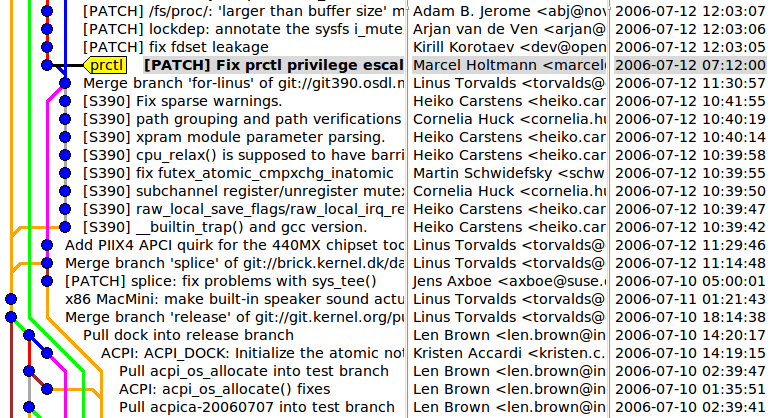
\includegraphics[width=12cm]{prctl}
\end{frame}

\begin{frame}
  \frametitle{A Git repository}
  \begin{itemize}
  \item A Git repository is a collection of
    \emph{refs}---\emph{branches} and \emph{tags}.
  \item A ref is a named mutable pointer to an object (usually a
    commit).
    \begin{itemize}
    \item \texttt{HEAD} $\to$ \texttt{refs/heads/master}
    \item \texttt{refs/heads/master} $\to$ \texttt{commit fec6ed\ldots}
    \item \texttt{refs/heads/ftrace} $\to$ \texttt{commit ce5c1e\ldots}
    \item \texttt{refs/tags/v2.6.8} $\to$ \texttt{commit e8ce2f\ldots}
    \item \texttt{refs/tags/v2.6.27} $\to$ \texttt{tag 4b5127\ldots}
    \end{itemize}
  \item The repository automatically stores the directed acyclic graph
    of objects rooted at these refs.
  \end{itemize}
\end{frame}

\section{Using Git}

\begin{frame}
  \frametitle{Outline}
  \tableofcontents[currentsection]
\end{frame}

\begin{frame}
  \frametitle{Getting a Git repository}

  \begin{description}[\texttt{git clone \textit{url}}]
  \item[\texttt{git init}] Create an empty Git repository in the
    current directory.  By default it will have one branch named
    \texttt{master}.
  \item[\texttt{git clone \textit{url}}] Clone the Git repository from
    \texttt{\textit{url}}.  This may be over HTTP, SSH, or the Git
    protocol, or it may be a path to another local repository.
  \end{description}

  Both of these operations will create a \emph{working copy}.
\end{frame}

\begin{frame}
  \frametitle{Working copy}
  \begin{itemize}
  \item Every working copy has its own Git repository in the
    \texttt{.git} subdirectory (with arbitrarily many branches and
    tags).
    \begin{itemize}
    \item The most important ref is \texttt{HEAD}, which refers to the
      current branch.
    \end{itemize}
  \item The \texttt{.git} subdirectory also stores the \emph{index}: a
    staging area for changes on top of \texttt{HEAD} that will become
    part of the next commit.
  \item Finally, the files outside of \texttt{.git} are the
    \emph{working tree}.
  \end{itemize}
\end{frame}

\begin{frame}
  \frametitle{Git workflow}
  \begin{itemize}
  \item Changes made to the working tree can be \emph{added} to the
    index.
  \item The index can be \emph{committed} to the current branch (where
    it will then become the new \texttt{HEAD}).
  \end{itemize}

  \begin{center}
    \includegraphics[width=9cm]{index}
  \end{center}
\end{frame}

\begin{frame}
  \frametitle{Constructing commits}
  \begin{description}[\texttt{git show \textit{object}}]
  \item[\texttt{git add \textit{file}}] Add or update
    \texttt{\textit{file}} from the working tree into the index.
  \item[\texttt{git reset \textit{file}}] Unstage changes to
    \texttt{\textit{file}} in the index, without touching the working
    copy.
  \item[\texttt{git rm \textit{file}}] Delete \texttt{\textit{file}}
    from the index and the working tree.
  \item[\texttt{git status}] Display the files changed in the index
    and in the working tree.
  \item[\texttt{git commit}] Make a commit out of the current index.
  \end{description}
\end{frame}

\begin{frame}
  \frametitle{Displaying changes}

  \begin{description}[\texttt{git diff --cached}]
  \item[\texttt{git log}] List the commits on the current branch.
  \item[\texttt{git show \textit{object}}] Show an object (e.g. a commit).
  \item[\texttt{git diff}] Show the differences between the index and
    the working tree.
  \item[\texttt{git diff --cached}] Show the differences between
    \texttt{HEAD} and the index.
  \item[\texttt{git diff \textit{commit}}] Show the differences
    between \textit{commit} and the working tree.
  \end{description}
\end{frame}

\begin{frame}
  \frametitle{Manipulating branches}

  \begin{description}[\texttt{git checkout -b \textit{branch}}]
  \item[\texttt{git branch}] List the branches in your repository,
    with the current branch highlighted.
  \item[\texttt{git checkout \textit{branch}}] Switch to the branch
    named \texttt{\textit{branch}}.  This updates \texttt{HEAD}, the
    index, and the working tree.
  \item[\texttt{git checkout -b \textit{branch}}] Create a new branch
    named \texttt{\textit{branch}} and switch to it.
  \end{description}
\end{frame}

\begin{frame}
  \frametitle{Merging}
  \begin{description}[\texttt{git merge \textit{branch}}]
  \item[\texttt{git merge \textit{branch}}] Merge
    \texttt{\textit{branch}} into \texttt{HEAD}. The index must not
    contain any staged changes.
  \end{description}

  \begin{itemize}
  \item A \emph{merge commit} is a commit with more than one parent.
  \end{itemize}

  \begin{center}
    \includegraphics[width=4cm]{merge}
  \end{center}
\end{frame}

\begin{frame}[fragile]
  \frametitle{Merging example}

  \hspace*{-0.5cm}
  \begin{tikzpicture}
    \useasboundingbox (0, 0) rectangle (11.5, 7);
    \begin{scope}
      \clip (0, 0) rectangle (11.5, 7);
      \draw (0, 0) node[anchor=south west,inner sep=0pt] {\vbox{\footnotesize
\begin{semiverbatim}
\only<1->{\sh{seq 5 > numbers}
}\only<2->{\sh{git init}
Initialized empty Git repository in /tmp/foo/.git/
}\only<3->{\sh{git add numbers}
}\only<4->{\sh{git commit -m '1, 2, 3, 4, 5!'}
Created initial commit 4172330: 1, 2, 3, 4, 5!
 1 files changed, 5 insertions(+), 0 deletions(-)
 create mode 100644 numbers
}\only<5->{\sh{git checkout -b andersk}
Switched to a new branch "andersk"
}\only<6->{\sh{git branch}
* {\color{green}andersk}
  master
}\only<7->{\sh{(echo 0; cat numbers) | sponge numbers}
}\only<8->{\sh{git diff}
\textbf{diff --git a/numbers b/numbers
index 8a1218a..e8371f0 100644
--- a/numbers
+++ b/numbers}
{\color{cyan}@@ -1,3 +1,4 @@}
{\color{green}+0}
 1
 2
 3
}\only<9->{\sh{git add numbers}
}\only<10->{\sh{git commit -m 'Numbers start at 0.'}
Created commit 7aeb494: Numbers start at 0.
 1 files changed, 1 insertions(+), 0 deletions(-)
}\only<11->{\sh{git checkout master}
Switched to branch "master"
}\only<12->{\sh{echo 6 >> numbers}
}\only<13->{\sh{git add numbers}
}\only<14->{\sh{git commit -m '6 is a number too.'}
Created commit 383c158: 6 is a number too.
 1 files changed, 1 insertions(+), 0 deletions(-)
}\only<15->{\sh{git merge andersk}
Auto-merged numbers
Merge made by recursive.
 numbers |    1 {\color{green}+}
 1 files changed, 1 insertions(+), 0 deletions(-)
}\only<16->{\sh{cat numbers}
0
1
2
3
4
5
6
}\only<17->{\sh{git checkout andersk}
Switched to branch "andersk"
}\only<18->{\sh{echo 5\textonehalf >> numbers}
}\only<19->{\sh{git add numbers}
}\only<20->{\sh{git commit -m '5\textonehalf is a better number.'}
Created commit 5360c2d: 5\textonehalf is a better number.
 1 files changed, 1 insertions(+), 0 deletions(-)
}\only<21->{\sh{git checkout master}
Switched to branch "master"
}\only<22->{\sh{git merge andersk}
Auto-merged numbers
CONFLICT (content): Merge conflict in numbers
Automatic merge failed; fix conflicts and then commit the result.
}\only<23->{\sh{git status}
numbers: needs merge
# On branch master
# Changed but not updated:
#   (use "git add <file>..." to update what will be committed)
#
#	{\color{red}unmerged:   numbers}
#
no changes added to commit (use "git add" and/or "git commit -a")
}\only<24->{\sh{git mergetool}
Merging the files: numbers

Normal merge conflict for 'numbers':
  {local}: modified
  {remote}: modified
Hit return to start merge resolution tool (meld): 
}\only<26->{\sh{cat numbers}
0
1
2
3
4
5
5\textonehalf
6
}\only<27->{\sh{git status}
# On branch master
# Changes to be committed:
#   (use "git reset HEAD <file>..." to unstage)
#
#	{\color{green}modified:   numbers}
#
# Untracked files:
#   (use "git add <file>..." to include in what will be committed)
#
#	{\color{red}numbers.orig}
}\only<28->{\sh{git commit}
Created commit fc8da7a: Merge branch 'andersk'
}
\end{semiverbatim}
      \vspace{-2em}}};
    \end{scope}
    \draw (12.5, 8.2) node[anchor=north east] {
      \only<4>{\includegraphics[width=8cm]{merge1}}%
      \only<5-9>{\includegraphics[width=8cm]{merge2}}%
      \only<10>{\includegraphics[width=8cm]{merge3}}%
      \only<11-13>{\includegraphics[width=8cm]{merge4}}%
      \only<14>{\includegraphics[width=8cm]{merge5}}%
      \only<15-16>{\includegraphics[width=8cm]{merge6}}%
      \only<17-19>{\includegraphics[width=8cm]{merge7}}%
      \only<20>{\includegraphics[width=8cm]{merge8}}%
      \only<21-27>{\includegraphics[width=8cm]{merge9}}%
      \only<28>{\includegraphics[width=8cm]{merge10}}%
    };
    \only<25>{\draw (current bounding box.center) node {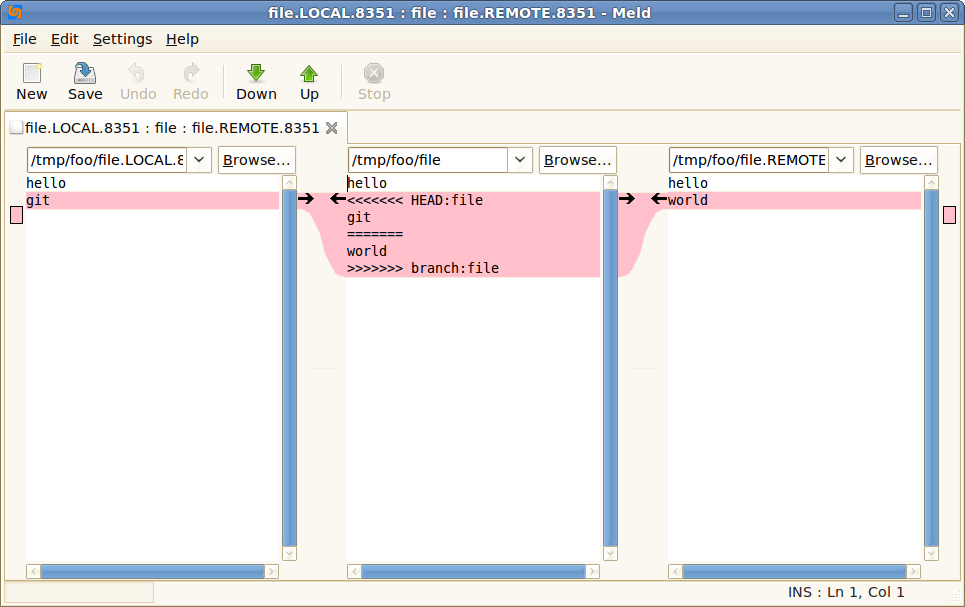
\includegraphics[width=11.5cm]{meld}};}
  \end{tikzpicture}
\end{frame}

\begin{frame}
  \frametitle{Rebasing}
  \begin{description}[\texttt{git rebase \textit{branch}}]
  \item[\texttt{git rebase \textit{branch}}] Rebase \texttt{HEAD} onto
    \texttt{\textit{branch}}.
  \end{description}

  \begin{center}
    \only<1>{\includegraphics[width=4cm]{rebase1}}
    \only<2>{\includegraphics[width=4cm]{rebase2}}
    \only<3>{\includegraphics[width=4cm]{rebase3}}
  \end{center}
\end{frame}

\end{document}
